\documentclass[dvipdfmx, titlepage, 11pt]{jsarticle}
\usepackage{tikz}
\usetikzlibrary{patterns}
\usetikzlibrary{intersections,calc,arrows}
\usepackage[top=20truemm,bottom=20truemm,left=15truemm,right=15truemm]{geometry}
\usepackage{enumerate}
\usepackage{multicol}
\usepackage{diagbox}
\usepackage{graphicx}

\makeatletter
\newcommand{\overarc}[1]{
  \setbox0\hbox{#1}%
  \ifdim\wd0<1em%
    \stackrel{\frown}{#1}%
  \else\ifdim\wd0<1.75em%
    \stackrel{\rotatebox{90}{\big)}}{#1}%
  \else\ifdim\wd0<2.5em%
    \stackrel{\rotatebox{90}{\Big)}}{#1}%
  \else\ifdim\wd0<3.25em%
    \stackrel{\rotatebox{90}{\bigg)}}{#1}%
  \else%
    \stackrel{%
      \rotatebox[origin=c]{90}{\mbox{%
        $\left.\vphantom{\rotatebox[origin=c]{90}{#1}}\right)$%
      }}%
    }{#1}%
  \fi\fi\fi\fi%
}
\makeatother

\newcommand{\ncircle}[1]{\textcircled{\scriptsize #1}}
\newcommand{\nbox}[1]{\fbox{\hspace{5pt} \textcircled{\scriptsize #1}\hspace{5pt} }}
\newcommand{\ebox}{\fbox{ \hspace{10pt} }}

\title{\Huge 数学}
\author{\LARGE 試験時間 : 50分}
\date{\LARGE 令和2年度筑波大附属高校\\[3cm] 大問は \fbox{\Large {\bf 1}} から \fbox{\Large {\bf 5}} まであります\\[0.5cm] 解答は解答用紙に記入して下さい}
\begin{document}
\maketitle

\newpage
\thispagestyle{empty}
 
\newpage

\newpage
\thispagestyle{empty}
 
\newpage

\setcounter{page}{1}
\noindent \fbox{\LARGE {\bf 1}}\hspace{10pt} 2個以上のさいころを投げたとき, 出た目すべての積の値を$a$とし, $a$の正の約数の個数について考える. \\
このとき, 次の \ncircle{1} 〜 \ncircle{3}の \ebox にあてはまる数を求めなさい. 
\begin{enumerate}[(1)]
\item 2個のさいころを投げるとき, $a$の正の約数の個数が \fbox{\hspace{5pt} \ncircle{1} -- ア\hspace{5pt} } 個となる確率が最も大きく, その確率は \fbox{\hspace{5pt} \ncircle{1} -- イ\hspace{5pt} } である.\\
  また, $a$の正の約数の個数が奇数個となる確率は \nbox{2} である.\\[7cm]
\item 3個のさいころを投げるとき, $a$の正の約数の個数が3個となるような$a$の値をすべて求めると, $a=$\ \nbox{3} である.
\end{enumerate}

\newpage

\begin{multicols}{2}
  \noindent \fbox{\LARGE {\bf 2}}\hspace{10pt} AB=3cm, BC=4cm, CA=5cmである$\triangle$ABCがある. 3点P,\ \ Q,\ \ Rはそれぞれの頂点A,\ \ B,\ \ Cを同時に出発して,\\
  \hspace{0.6cm} 点Pは毎秒3cmの速さで, A$\to$B$\to$C$\to$A$\to\ \cdots$\\
  \hspace{0.6cm} 点Qは毎秒2cmの速さで, B$\to$C$\to$A$\to$B$\to\ \cdots$\\
  \hspace{0.6cm} 点Rは毎秒1cmの速さで, C$\to$A$\to$B$\to$C$\to\ \cdots$\\
  のようにすべて同じ向きに進み, 3点がそれぞれの最初の位置に同時に戻ったとき, 3点とも止まる.\\
  3点が出発してからの時間を$x$秒とするとき 次の \ncircle{4} 〜 \ncircle{6} の \ebox \ にあてはまる数または式を求めなさい.
  \begin{center}
    $\langle\langle$計算欄$\rangle\rangle$\\[0.1cm]
    
    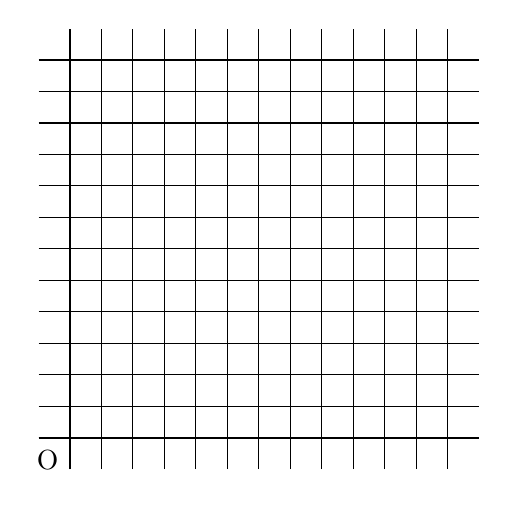
\begin{tikzpicture}[scale=0.4]
      \draw (-0.99,-0.99) grid (12.99, 12.99);
      \draw[thick] (0,-0.99)--(0,12.99);
      \draw[thick] (-0.99,0)--(12.99,0);
      \node at (-0.7,-0.7) {O};
    \end{tikzpicture}
  \end{center}
\end{multicols}
\begin{enumerate}[(1)]
\item $x>0$のとき, 3点が動いている間にP,\ \ Q,\ \ Rがつくる三角形$\triangle$ABCと合同になるときの$x$の値と, 3点が止まるときの$x$の値を求めると, $x=$ \nbox{4} である.\\[3cm]
\item 3点P,\ \ Q,\ \ Rのうち, 2つの点が重なることは \nbox{5} 回ある.\\[3cm]
\item 3点P,\ \ Q,\ \ Rが三角形をつくらない時間すべてを, $x$についての等式または不等式で表すと, \nbox{6} である.
\end{enumerate}
\newpage

\begin{minipage}{0.6\hsize}
  \noindent \fbox{\LARGE {\bf 3}}\hspace{10pt} 右の図のように, 線分BC上に点DをBD : DC = 2:3となるようにとり, 線分BCに垂直な線分DAを$\angle$BAC=45${}^{\circ}$となるように引く.\\
  このようにしてできた$\triangle$ABCに対して頂点Bから辺ACに垂直な線分BEを引き, ADとBEの交点をHとする.\\
  このとき, 次の\ncircle{7} 〜 \ncircle{9} の \ebox \ にあてはまる三角形または数を求めなさい.
\end{minipage}
\begin{minipage}{0.36\hsize}
  \begin{center}
    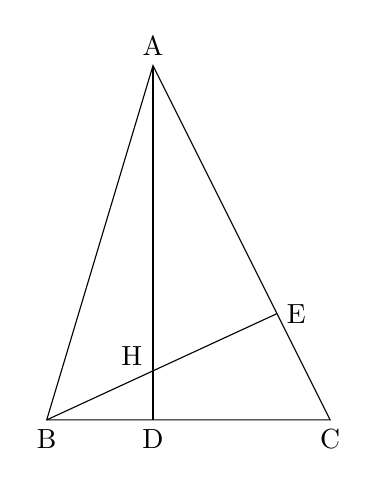
\begin{tikzpicture}[scale=0.9]
      \draw (0,0) node[below] {B}--(4,0)node[below] {C}--(1.5,5)node[above] {A}--cycle;
      \draw[name path =A] (1.5,5)--(1.5,0)node[below] {D};
      \draw[name path =B] (0,0)--(3.25,1.5)node[right] {E};
      \node at (1.2,0.9) {H};
    \end{tikzpicture}
  \end{center}
\end{minipage}

\begin{enumerate}[(1)]
\item $\triangle$BCEと相似な三角形のうち, $\triangle$BCE以外のものを2つあげると, \nbox{7} である.\\[1cm]
\item 線分AHの長さは, 線分BDの長さの \nbox{8} 倍である.\\[6cm]
\item AH=10cmであるとき, $\triangle$ABCの面積は, \nbox{9} cm${}^{2}$である.
\end{enumerate}
\newpage
 
\newpage
\begin{minipage}{0.7\hsize}
  \noindent \fbox{\LARGE {\bf 4}}\hspace{10pt} ふたがついた大きさの異なる2つの直方体の箱X,\ \ Yがある. Xには半径$r$cmの球が5個, Yには半径4cmの球が4個, 底面に接するように入っている.
\end{minipage}
\begin{minipage}{0.29\hsize}
  \begin{center}
    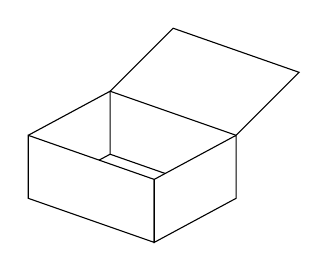
\begin{tikzpicture}[scale=0.8]
      \draw (0,0)--(1.3,0.7)--(1.3,1.7)--(0,1);
      \draw (1.3,0.7)--(3.3,0);
      \draw (1.3,1.7)--(3.3,1);
      \draw[fill=white] (0,0)--(2,-0.7)--(2,0.3)--(0,1)--cycle;
      \draw[fill=white] (2,-0.7)--(3.3,0)--(3.3,1)--(2,0.3)--cycle;

      \draw (1.3,1.7)--(2.3,2.7)--(4.3,2)--(3.3,1);
    \end{tikzpicture}
  \end{center}
\end{minipage}
下の図1の長方形ABCD,\ \ EFGHはそれぞれX,\ \ Yの平面図であり, AD=EHである.
\begin{multicols}{2}
  \begin{center}
    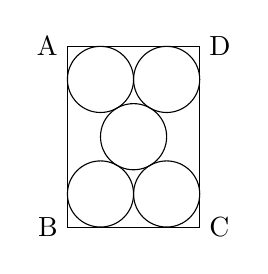
\begin{tikzpicture}[scale=1.4]
      \draw (0,0) circle[radius=0.3];
      \draw (60:0.6) circle[radius=0.3];
      \draw (120:0.6) circle[radius=0.3];
      \draw (240:0.6) circle[radius=0.3];
      \draw (300:0.6) circle[radius=0.3];
      \draw ($(240:0.6)+(-0.3,-0.3)$) node[left] {B} rectangle ($(60:0.6)+(0.3,0.3)$) node[right] {D};
      \draw ($(120:0.6)+(-0.3,0.3)$) node[left] {A};
      \draw ($(300:0.6)+(0.3,-0.3)$) node[right] {C};
    \end{tikzpicture}

    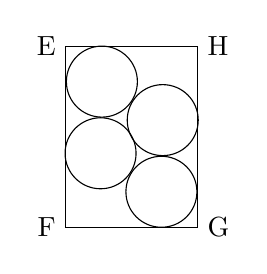
\begin{tikzpicture}[scale=1.4]
      \draw ($(120:0.6)+(0.03,-0.02)$)circle[radius=0.322];
      \draw ($(300:0.6)+(-0.03,0.02)$) circle[radius=0.322];
      \draw ($(300:0.6)+(-0.018,0.67)$) circle[radius=0.322];
      \draw ($(120:0.6)+(0.018,-0.67)$) circle[radius=0.322];
      
      \draw ($(240:0.6)+(-0.3,-0.3)$) node[left] {F} rectangle ($(60:0.6)+(0.3,0.3)$) node[right] {H};
      \draw ($(120:0.6)+(-0.3,0.3)$) node[left] {E};
      \draw ($(300:0.6)+(0.3,-0.3)$) node[right] {G};
    \end{tikzpicture}
  \end{center}
\end{multicols}
\centerline{(図1)}

図1のように, 隣り合う球は互いに接しており, それぞれの箱の4個の球は側面に接している. このとき, 次に \ncircle{10} 〜 \ncircle{12}の \ebox \ にあてはまる数または辺を求めなさい.
\begin{enumerate}[(1)]
\item $r=$ \nbox{10} cmである.\\[6cm]
\item 辺ABと辺EFの長さを比べると, 辺 \fbox{\hspace{5pt} \ncircle{11} -- ア\hspace{5pt} } の方が \fbox{\hspace{5pt} \ncircle{11} -- イ\hspace{5pt} } cm だけ長い.
  \newpage
  
  \begin{multicols}{2}
  \item 右の図2のように, Xには半径$r$cmの球, Yには半径4cmの球をそれぞれの3個の球と接するように1個ずつ置き, ふたをして直方体にしたところ, どちらのふたも置いた球と接した.\\
    このとき, Xの体積は, Yの体積の \nbox{12} 倍である.

    \begin{center}
      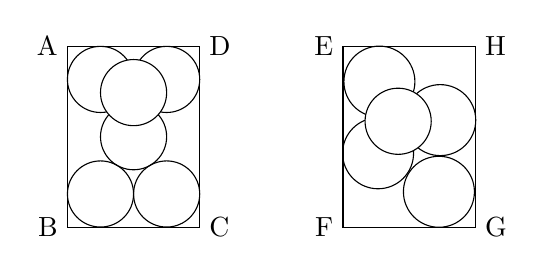
\begin{tikzpicture}[scale=1.4]
        \draw (0,0) circle[radius=0.3];
      \draw (60:0.6) circle[radius=0.3];
      \draw (120:0.6) circle[radius=0.3];
      \draw (240:0.6) circle[radius=0.3];
      \draw (300:0.6) circle[radius=0.3];
      \draw[fill=white] (0,0.4) circle[radius=0.3];
      \draw ($(240:0.6)+(-0.3,-0.3)$) node[left] {B} rectangle ($(60:0.6)+(0.3,0.3)$) node[right] {D};
      \draw ($(120:0.6)+(-0.3,0.3)$) node[left] {A};
      \draw ($(300:0.6)+(0.3,-0.3)$) node[right] {C};

      
      \draw ($(2.5,0)+(120:0.6)+(0.03,-0.02)$)circle[radius=0.322];
      \draw ($(2.5,0)+(300:0.6)+(-0.03,0.02)$) circle[radius=0.322];
      \draw ($(2.5,0)+(300:0.6)+(-0.018,0.67)$) circle[radius=0.322];
      \draw ($(2.5,0)+(120:0.6)+(0.018,-0.67)$) circle[radius=0.322];
      \draw[fill=white] (2.4,0.14) circle[radius=0.3];

      
      \draw ($(2.5,0)+(240:0.6)+(-0.3,-0.3)$) node[left] {F} rectangle ($(2.5,0)+(60:0.6)+(0.3,0.3)$) node[right] {H};
      \draw ($(2.5,0)+(120:0.6)+(-0.3,0.3)$) node[left] {E};
      \draw ($(2.5,0)+(300:0.6)+(0.3,-0.3)$) node[right] {G};
      \end{tikzpicture}

      (図2)
    \end{center}
  \end{multicols}
\end{enumerate}



\newpage
\noindent \fbox{\LARGE {\bf 5}}\hspace{10pt} 「$1+2\times 3+4=$」と入力すると, 計算結果が11となる電卓を使用する.\\
このとき, 次の \ncircle{13},\ \ \ncircle{14} の \ebox \ にあてはまる数または数の組を求めなさい. ただし, 1から10までの連続する自然数の和$1+2+3+\cdots\cdots+10$は, 55である.
\begin{enumerate}[(1)]
\item 11から20までの連続する10個の自然数を小さい方から順に入力して和を計算しようとしたところ, 自然数$n$の次の「+」を「$\times$」と押し間違えてしまい, 計算結果が364となった. このとき, $n=$ \nbox{13} である.\\[6cm]
\item 自然数$m$から$m+9$までの連続する10個の自然数を小さい方から順に入力して和を計算しようとしたところ, 自然数$n$の次の「+」を「$\times$」と押し間違えてしまい, 計算結果が94となった.\\
  このような自然数の組$(m,\ n)$をすべて求めると, \nbox{14} である. なお, \ncircle{14} の解答欄には答えを求めるまでの過程や考え方も書きなさい.
\end{enumerate}
\newpage
\thispagestyle{empty}
 
\newpage
\newpage
\thispagestyle{empty}
 
\newpage

\end{document}
